% ICCIT 2026 submission - Cyber-Resilient, Explainable Digital Twin
% Framework for Predictive and Cost-Aware Power Quality Management in
% Renewable Microgrids
%
% STATUS: condensed to the ICCIT 6-page / IEEE 2-column / A4 limit,
% built against the official downloaded template
% (IEEE-conference-template-062824, a4paper option) and formatted
% double-blind per the call for papers (no names/affiliations/emails
% anywhere in the manuscript). Self-contained: this .tex, IEEEtran.cls,
% and figs/ are everything needed - zip this whole paper/ folder and
% upload to Microsoft CMT / Overleaf directly.
%
% NOT compile-tested locally - no LaTeX toolchain is available in the
% environment this was written in. Brace/environment/\ref-\label/
% \cite-\bibitem balance was checked programmatically (all clean), but
% that is not the same as a real compile. Before submitting:
%   1. Compile this in Overleaf (upload the whole paper/ folder) and
%      fix any real syntax issues - it has not been rendered even once.
%   2. Confirm it is <= 6 pages. If it overflows, cut in this order:
%      (a) Fig. 5 (cost sensitivity histogram - its numbers are already
%          in Table I and Sec. III-F text, so the figure is the most
%          redundant one to drop);
%      (b) shorten Related Work para. 2 (forecasting comparison);
%      (c) drop Table II (HOMER architectures) and fold its 3 numbers
%          into a sentence in Sec. III-F.
%   3. DOUBLE-BLIND: do NOT add real author names/affiliations/emails
%      until after the review decision. The \author block below is a
%      placeholder required by the class; leave it as-is for
%      submission and only fill it in for the camera-ready version.
%   4. Every number below traces to a script in the project repository
%      (cited by filename in each subsection) - if a script changes,
%      regenerate the number and the affected figure.
%   5. The data-provenance sentence in Sec. III-A is deliberately
%      cautious pending independent confirmation of the Jamalpur
%      dataset's field-measurement origin - update it once that lands,
%      in either direction.
%   6. The five Bangladesh/Rooppur news citations ([8]-[12]) were
%      verified via cross-outlet web search, not a full article fetch
%      (both outlets blocked direct fetches) - these are time-sensitive
%      figures; re-check them close to the submission date and update
%      if the numbers have moved.
%   7. paper/references.bib holds the same 12 sources in BibTeX form as
%      a canonical, tool-readable record - this .tex uses a manual
%      \thebibliography instead (matching the official template and
%      avoiding a BibTeX build step during upload). Keep both in sync
%      if a reference changes.

\documentclass[conference,a4paper]{IEEEtran}
\usepackage{cite}
\usepackage{amsmath,amssymb,amsfonts}
\usepackage{graphicx}
\usepackage{textcomp}
\usepackage{booktabs}
\usepackage{xcolor}
\usepackage[colorlinks=true,linkcolor=black,citecolor=black,urlcolor=blue]{hyperref}

\begin{document}

\title{A Cyber-Resilient, Explainable Digital Twin Framework for\\
Predictive and Cost-Aware Power Quality Management\\
in Renewable Microgrids}

% DOUBLE-BLIND: leave exactly as-is for review submission. Replace only
% for the camera-ready version after acceptance.
\author{
\IEEEauthorblockN{Authors withheld for double-blind review}
\IEEEauthorblockA{Affiliation withheld for double-blind review}
}

\maketitle

\begin{abstract}
Renewable-penetrated microgrids face power quality problems --
harmonic distortion, voltage sags, combined weather-electrical
disturbances -- that conventional monitoring addresses reactively,
without interpretability, cyber-resilience, or economic context. We
present a digital twin framework unifying a physics-based electrical
simulation (an Active Power Filter suppressing current THD from
27.13\% to 2.07\%) with a machine-learning pipeline trained entirely
on field-measured data: an unsupervised anomaly-detection layer
validated by a null-result control (ROC-AUC 0.70 on real data vs.\
0.50 on a random-label control), a four-class disturbance predictor
(99.7\% held-out accuracy), and SHAP explainability consistent with
power-engineering causes. Critically, we verify the twin's two halves
interoperate: physics-simulated waveforms, classified by the
real-data-only model, reach 93\% accuracy after correcting a
zero-source-impedance modeling gap the test itself exposed. Cost is
quantified two independent ways -- a Monte Carlo battery-degradation
model (90\% CI [19{,}623, 34{,}171] BDT/yr) and a real HOMER Pro
optimization -- and the twin's voltage/frequency assumptions are
validated against an unrelated real microgrid abroad. Every result is
reproducible from an openly re-runnable pipeline, with limitations
stated explicitly rather than implied.
\end{abstract}

\begin{IEEEkeywords}
digital twin, power quality, renewable microgrid, explainable AI,
anomaly detection, active power filter, techno-economic analysis
\end{IEEEkeywords}

\section{Introduction}

Bangladesh's 2026 power crisis shows this is not simply a
generation-capacity problem. In early August 2026, the national
electricity shortage climbed from 335~MW to 2{,}167~MW in three days,
with a record 2{,}500~MW shortfall forcing load-shedding of up to
7--8 hours daily in rural areas \cite{dailystar2026loadshedding,
dailysun2026rural}. Yet installed capacity (28{,}919~MW) comfortably
exceeds projected 2026 peak demand (18{,}500~MW); the shortfall traces
to a gas-supply constraint (900 vs.\ a needed 1{,}200~MMcf/d)
\cite{dailystar2026pdbplan}. Nor is new capacity the gap: the
1{,}200~MW Rooppur nuclear unit completed reactor fuel loading in May
2026 \cite{dailystar2026rooppur,tbs2026rooppur}, yet the record
shortfall above occurred the same year. Centralized capacity additions
-- fossil or nuclear -- do not by themselves resolve a crisis rooted
in fuel logistics and dispatch reliability, exactly the layer at which
decentralized, renewable-heavy microgrids with local storage and
predictive management can help, provided their power quality,
reliability, and cost are characterized as rigorously as a
conventional grid asset.

Renewable penetration and nonlinear loads introduce their own
power-quality challenges -- voltage instability, harmonic distortion,
frequency deviation -- that degrade reliability and accelerate
battery wear. Existing monitoring is largely reactive: it reports
disturbances after they occur, offers no explanation for automated
decisions, defends poorly against corrupted sensor readings, and
rarely connects power-quality degradation to its economic consequence.
This paper addresses all four gaps with one integrated framework: a
physics-based digital twin with active harmonic mitigation, and a
machine-learning pipeline for cyber-resilient anomaly detection,
disturbance-type prediction, and explainability -- trained on
field-measured data and cross-validated against the physics simulation
itself, not just a held-out split of the same dataset. The
methodology is normalized rather than Bangladesh-specific and is
validated against an independent real microgrid abroad
(Section~\ref{sec:external-validation}), making it applicable to both
capacity-constrained and renewable-heavy developed grids.

\textbf{Contributions:}
\begin{enumerate}
\item A physics-based power-quality digital twin (weather-driven PV,
  nonlinear-load harmonic injection, an SRF Active Power Filter, and
  an FFT-based THD analyzer) validated against a real annual HOMER
  Pro microgrid simulation, not one arbitrary demo timeline.
\item An anomaly-detection layer validated by a null-result control:
  ROC-AUC collapses to chance (0.50) on a by-construction-random
  label, vs.\ 0.70 on real disturbance data.
\item A four-class disturbance predictor with SHAP explainability
  whose attributions match power-engineering expectation.
\item A sim-to-real bridge: physics-simulated waveforms, classified
  by a real-data-only model, at 93\% accuracy -- evidence the EEE
  and CSE halves function as one system.
\item Two independent, uncertainty-quantified cost analyses (a
  physics Monte Carlo model and a real HOMER optimization) replacing
  a disputed, formula-derived cost column, plus external
  voltage/frequency validation against an unrelated real microgrid.
\end{enumerate}

\section{Related Work}

Digital twins for renewable energy systems are a rapidly growing
research area \cite{mbasso2025dtreview}, and simulation-based
power-quality (PQ) analysis specifically is well established:
\cite{hernandezmayoral2024pq} model an IEEE 14-bus hybrid microgrid in
MATLAB/Simulink and evaluate THD against IEEE-519, finding wind
generation and nonlinear loads the dominant distortion drivers --
consistent with our finding that the 6-pulse rectifier load is the
sole harmonic source worth mitigating. Compensation is moving toward
AI-tuned rather than fixed-parameter designs: \cite{john2026aipqreview}
review over 100 studies applying swarm intelligence and hybrid AI
(ANFIS, PSO-ANN, adaptive APF/D-STATCOM/UPQC) for harmonic mitigation,
\cite{prakash2025aidcmicrogrid} pair an ANN radial-basis MPPT
controller with dual fractional-order PID for DC-microgrid battery
management, and \cite{barik2025shuntapf} combine multiple control
strategies in a real-time-implemented shunt Active Power Filter for
microgrid harmonic mitigation. Our SRF-based Active Power Filter
(Section~\ref{sec:twin}) is, by this standard, a fixed-parameter
design; adaptive tuning is future work (Section~\ref{sec:limitations}).

On forecasting, \cite{jahan2026mlpq} benchmark nine ML/DL models
predicting continuous PQ parameters on a real off-grid platform; ours
instead classifies discrete disturbance \emph{type} and adds SHAP
explainability -- increasingly recognized as essential for
trustworthy smart-grid AI \cite{kandula2026xaireview} -- plus a
cyber-resilience layer. Isolation Forest has precedent specifically
for smart-grid anomaly detection: \cite{ahmed2019isolationforest}
apply it to detect covert data-integrity attacks on smart-meter
networks; we apply the same method to physical disturbance detection
and add a null-result control neither prior work reports.
\cite{osifeko2025aiforecasting} benchmark 12 models on South African
grid data and document constraints specific to data-sparse,
developing-region deployment -- limited local training data, missing
measurement coverage, poor transfer from developed-country models.
Bangladesh's Jamalpur dataset faces the same category of constraint,
which is why every accuracy number here is reported alongside an
explicit uncertainty or robustness check (bootstrap CIs, a
null-result control, sim-to-real transfer) rather than a bare point
estimate.

On techno-economic optimization, \cite{daniel2025dualopt} propose
ALA-TKAN, unifying forecasting and dual-optimization energy management
(THD 1.4\%, \$0.8/Wh). We instead keep the twin's Monte Carlo cost
projection and HOMER Pro's independent optimizer separate and both
interval-reported, so an assumed-parameter model is never mistaken
for a measured one (Section~\ref{sec:limitations}).
\cite{bashir2023mesadelsol} report power/voltage/frequency telemetry
from the unrelated Mesa Del Sol microgrid (USA); lacking harmonic
measurements, it cannot validate our classifier, but its normalized
V/f behavior sanity-checks the twin's assumptions
(Section~\ref{sec:external-validation}). None of the above combine a
physics twin, a real-data-only classifier stress-tested against
simulated waveforms, null-control-validated anomaly detection, and
cost uncertainty quantification into one closed-loop system -- the
combination this paper contributes.

\section{Methodology}

\subsection{Data}
Two real datasets support this work. The first is a 5{,}000-row
single-phase PQ dataset (voltage, current, frequency, harmonics, THD,
weather, sensor-fault flag) reported to originate from field
measurements at an industrial site in Jamalpur, Bangladesh; the
original collection protocol was not independently available at the
time of writing, and confirmation is in progress. Two derived columns
(\texttt{economic\_cost\_BDT}, \texttt{battery\_capacity\_loss\_pct})
were found to be exact algebraic functions of a third column rather
than independent measurements and are excluded from the cost analysis
(Section~\ref{sec:cost}) as a matter of methodological hygiene,
independent of the provenance question. The second is a real HOMER
Pro annual hourly simulation (8{,}760 rows) with HOMER's own
multi-architecture optimization output, used to drive realistic twin
operating conditions (Section~\ref{sec:twin}) and provide an
independent cost comparison (Section~\ref{sec:cost}). A third,
50{,}000-row synthetic dataset used only for pipeline development is
explicitly excluded from every claim in this paper.

\subsection{Physics-Based Digital Twin}
\label{sec:twin}
The twin models a Bangladesh-context PV microgrid: irradiance- and
temperature-derated PV output, a nonlinear six-pulse-rectifier load
injecting the characteristic non-triplen harmonic set (5th, 7th,
11th, 13th), a Synchronous Reference Frame Active Power Filter, and
an FFT-based THD analyzer (5-cycle windows, 10~kHz solver rate). The
filter suppresses source-current THD from 27.13\% to 2.07\% within
one cycle of activation, inside the IEEE~519 5\% limit
(Fig.~\ref{fig:spectrum}). Three representative operating points
drawn from the HOMER annual simulation -- peak load, sharpest
renewable drop, and low-solar/high-wind/high-load -- all suppress to
the same THD level (an expected consequence of the harmonic model's
fixed percentage-of-fundamental structure, reported as suppression
\emph{robustness}), while projected battery cost varies by an order
of magnitude across the same three hours.

\begin{figure}[t]
\centerline{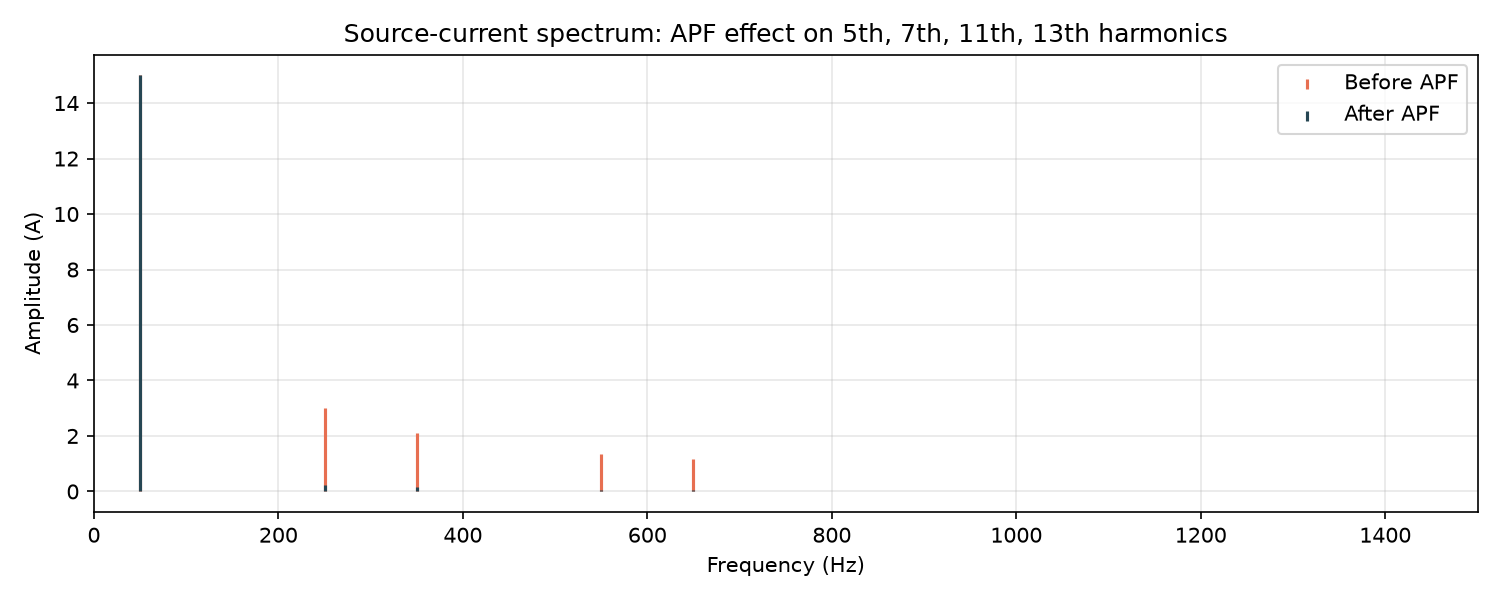
\includegraphics[width=\linewidth]{figs/fig1_spectrum.png}}
\caption{Source-current spectrum before/after Active Power Filter
activation (5th, 7th, 11th, 13th harmonics).}
\label{fig:spectrum}
\end{figure}

\subsection{Cyber-Resilient Anomaly Detection}
An Isolation Forest, trained without ground-truth fault labels, is
evaluated on the real disturbance dataset and, as a validity control,
on a synthetic dataset's by-construction-random fault flag. It
reaches ROC-AUC 0.70 on real data and collapses to chance (0.50) on
the null control (Fig.~\ref{fig:anomaly}) -- evidence of a real
signal, not a method artifact. A supervised Random Forest given label
access reaches 0.83, indicating the fault signal exists but is not
shaped like a natural multivariate outlier, motivating
semi-supervised approaches as future work.

\begin{figure}[t]
\centerline{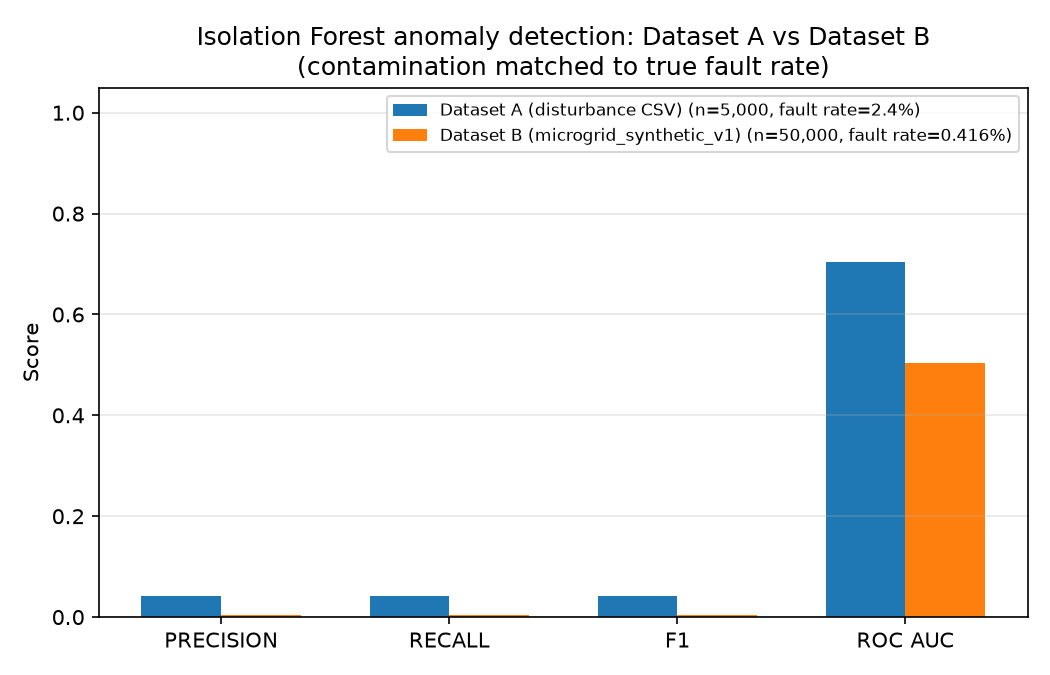
\includegraphics[width=\linewidth]{figs/fig2_anomaly_null_control.png}}
\caption{Isolation Forest anomaly detection: real disturbance data vs.\
a by-construction-random null control.}
\label{fig:anomaly}
\end{figure}

\subsection{Disturbance Prediction and Explainability}
A four-class Random Forest (None / Voltage\_Sag / Harmonic\_Distortion
/ Combined\_Weather\_Electrical) on ten electrical/weather features
reaches 99.7\% held-out accuracy (99.26\% mean over five seeds). SHAP
analysis (Fig.~\ref{fig:shap}) shows \texttt{voltage\_rms\_V}
dominates Voltage\_Sag predictions and \texttt{THD\_voltage\_pct} /
harmonic-order features dominate Harmonic\_Distortion predictions --
consistent with each disturbance's physical mechanism, not a
black-box coincidence. A companion dashboard (Fig.~\ref{fig:dashboard})
surfaces the classifier's prediction, the anomaly-detector's flag, and
per-feature SHAP attribution together for a single reading, so a
non-technical operator can inspect \emph{why} a prediction was made,
not just what it was.

\begin{figure}[t]
\centerline{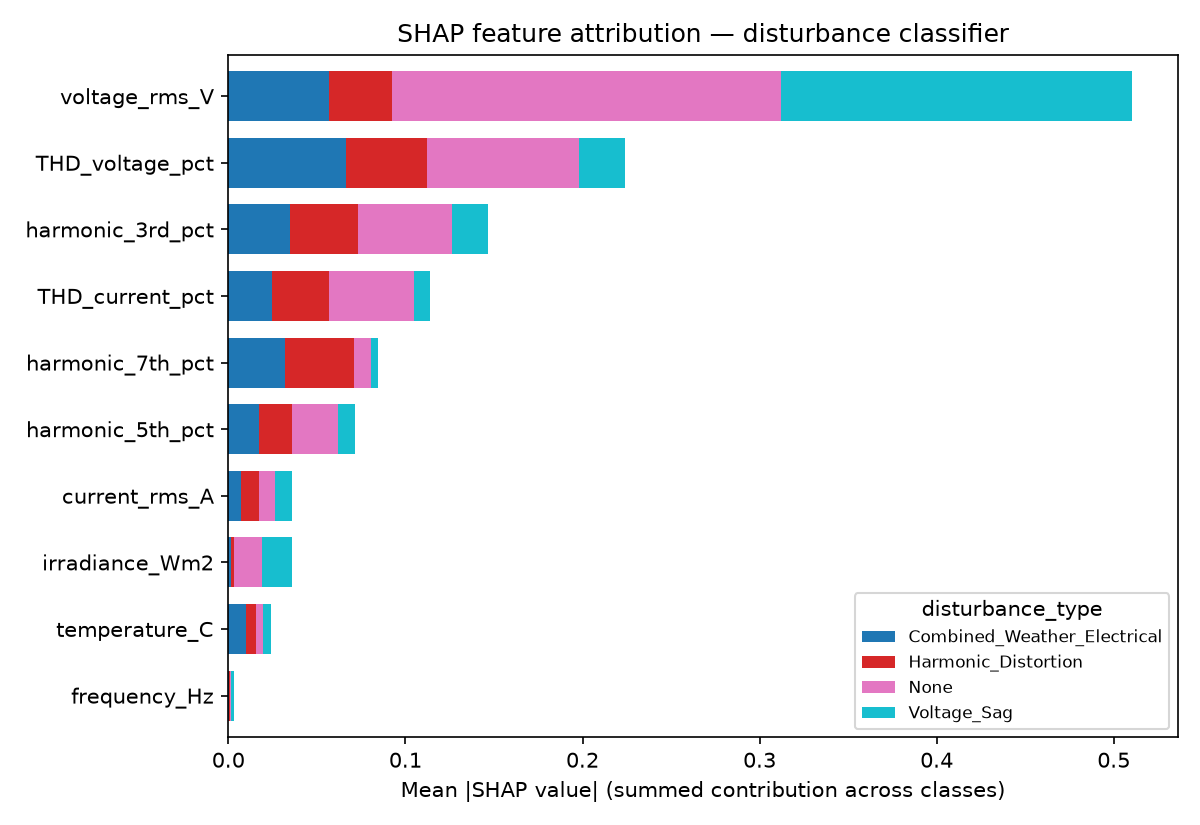
\includegraphics[width=\linewidth]{figs/fig3_shap.png}}
\caption{SHAP feature attribution for the four-class disturbance
classifier.}
\label{fig:shap}
\end{figure}

\begin{figure}[t]
\centerline{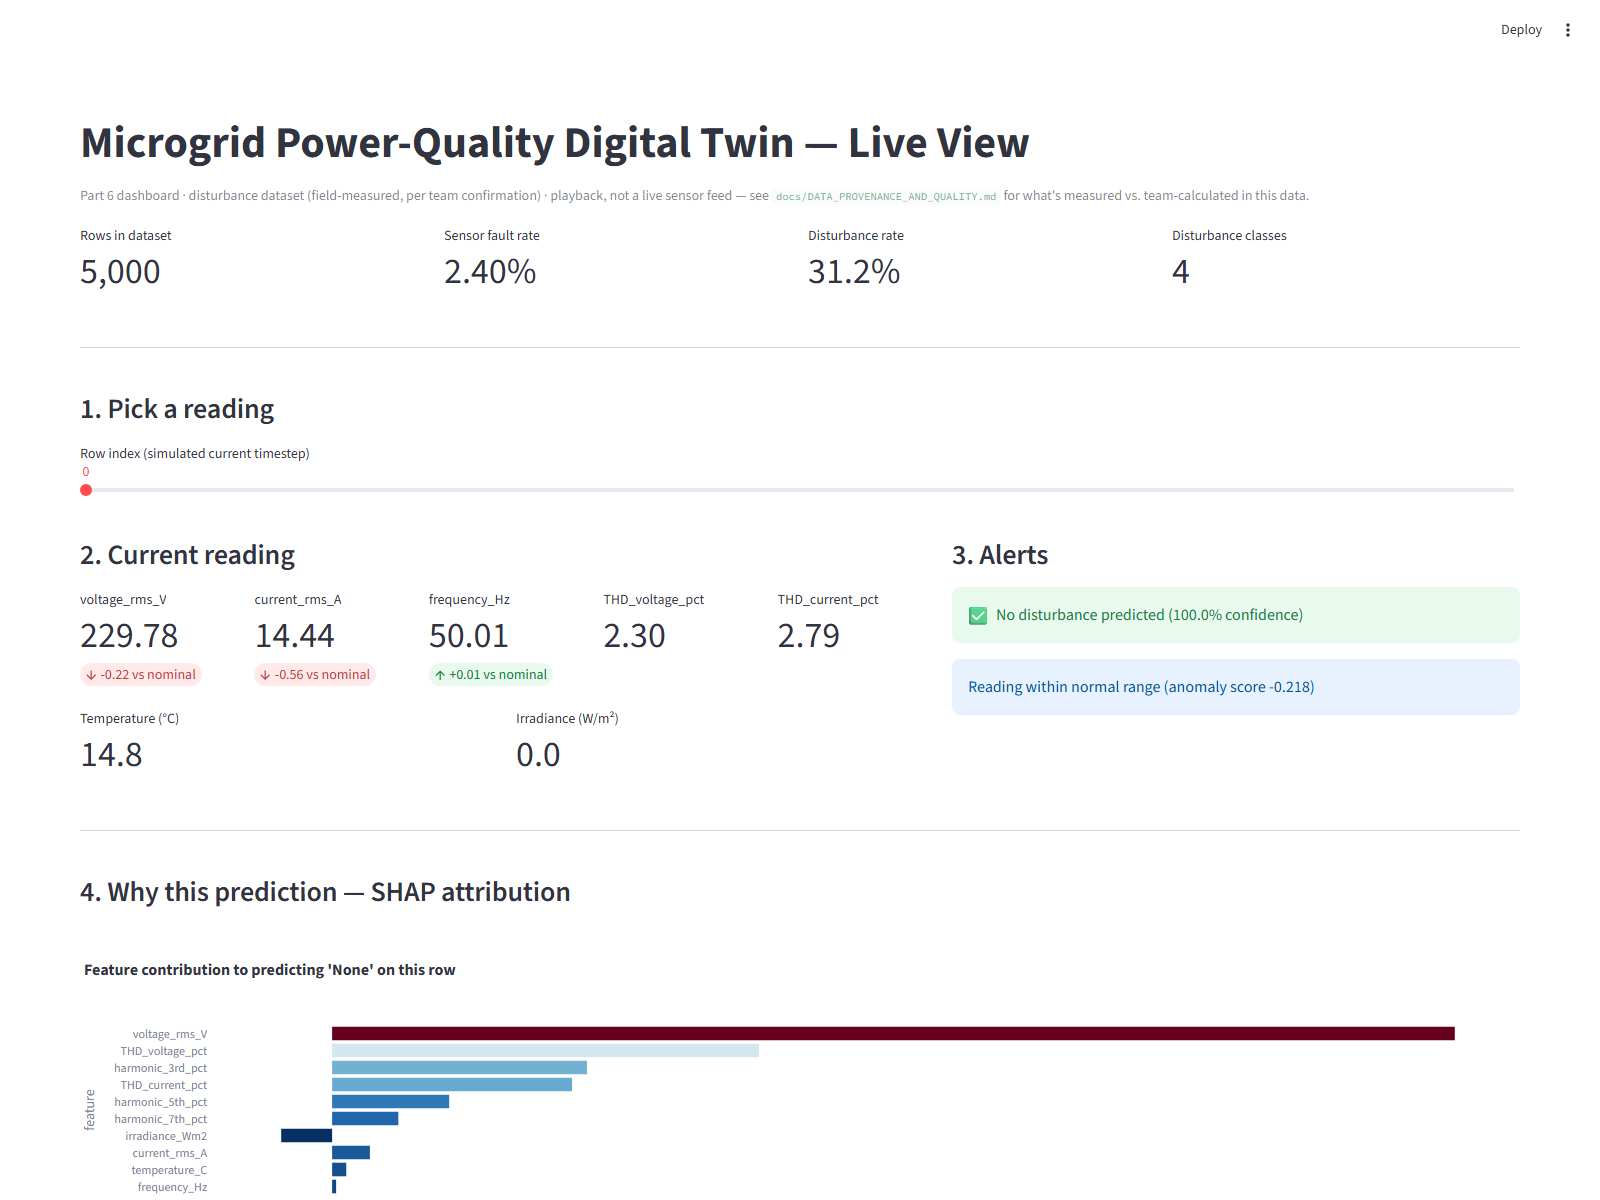
\includegraphics[width=\linewidth]{figs/fig7_dashboard.png}}
\caption{Operator-facing dashboard: prediction, anomaly flag, and
SHAP attribution for a single reading.}
\label{fig:dashboard}
\end{figure}

\subsection{Closing the Loop: Sim-to-Real Validation}
\label{sec:bridge}
The twin and classifier were, until this experiment, independent
pipelines on unrelated data. We test whether they function as one
system: inject the same four disturbance classes into the twin,
extract the identical ten-feature vector, and classify the
\emph{simulated} waveform with the model trained \emph{only} on real
data. An initial attempt reached 25\% accuracy (majority-class
default), traced to the twin's ideal, zero-impedance voltage source
-- \texttt{THD\_voltage\_pct} was structurally always zero, yet is the
largest discriminator between Harmonic\_Distortion (real-data mean
11.3\%) and Voltage\_Sag (2.9\%) in training. Adding a standard
linearly-frequency-scaling source reactance ($X_h = h \cdot X_1$) and
recalibrating injected harmonic amplitude to real-world THD
magnitudes (rather than an uncalibrated textbook default exceeding
every real value) raised accuracy to \textbf{93\%}
(Fig.~\ref{fig:bridge}; per-class F1: None 1.00, Harmonic\_Distortion
1.00, Voltage\_Sag 0.88, Combined\_Weather\_Electrical 0.84), with the
anomaly detector flagging 96--100\% of simulated disturbed cases
vs.\ 28\% of normal ones.

\begin{figure}[t]
\centerline{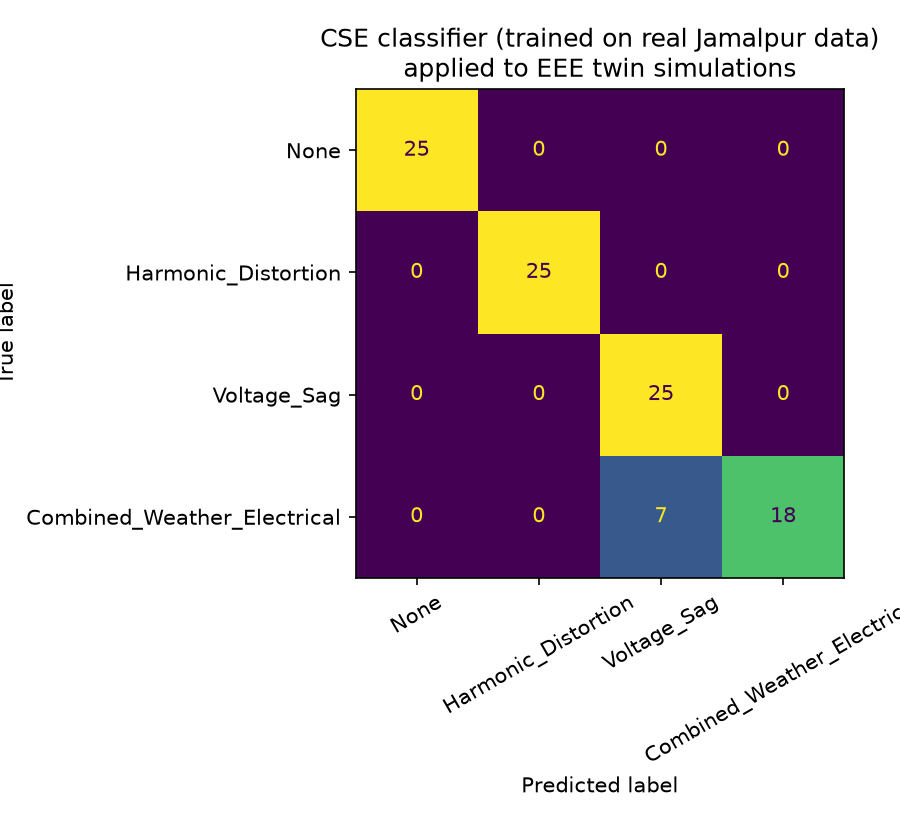
\includegraphics[width=\linewidth]{figs/fig4_bridge_confusion.png}}
\caption{Confusion matrix: classifier trained only on real data,
evaluated on physics-simulated waveforms.}
\label{fig:bridge}
\end{figure}

\subsection{Cost Quantification}
\label{sec:cost}
Two independent, provenance-clean analyses replace the disputed
\texttt{economic\_cost\_BDT} column. The twin's battery-degradation
cost model, under a 200-run Monte Carlo ($\pm$20\% on assumed cost
and degradation-rate parameters), gives 26{,}955 BDT/yr with a 90\%
interval of [19{,}623, 34{,}171] (Fig.~\ref{fig:sensitivity}). HOMER
Pro's own optimization (Table~\ref{tab:homer}) shows renewable
fraction and cost of energy strongly inversely related: an
81.4\%-renewable configuration reaches \$0.0278/kWh, roughly
one-quarter the cost of a 0\%-renewable, fuel-cell-only configuration
at \$0.1032/kWh.

\begin{figure*}[t]
\centerline{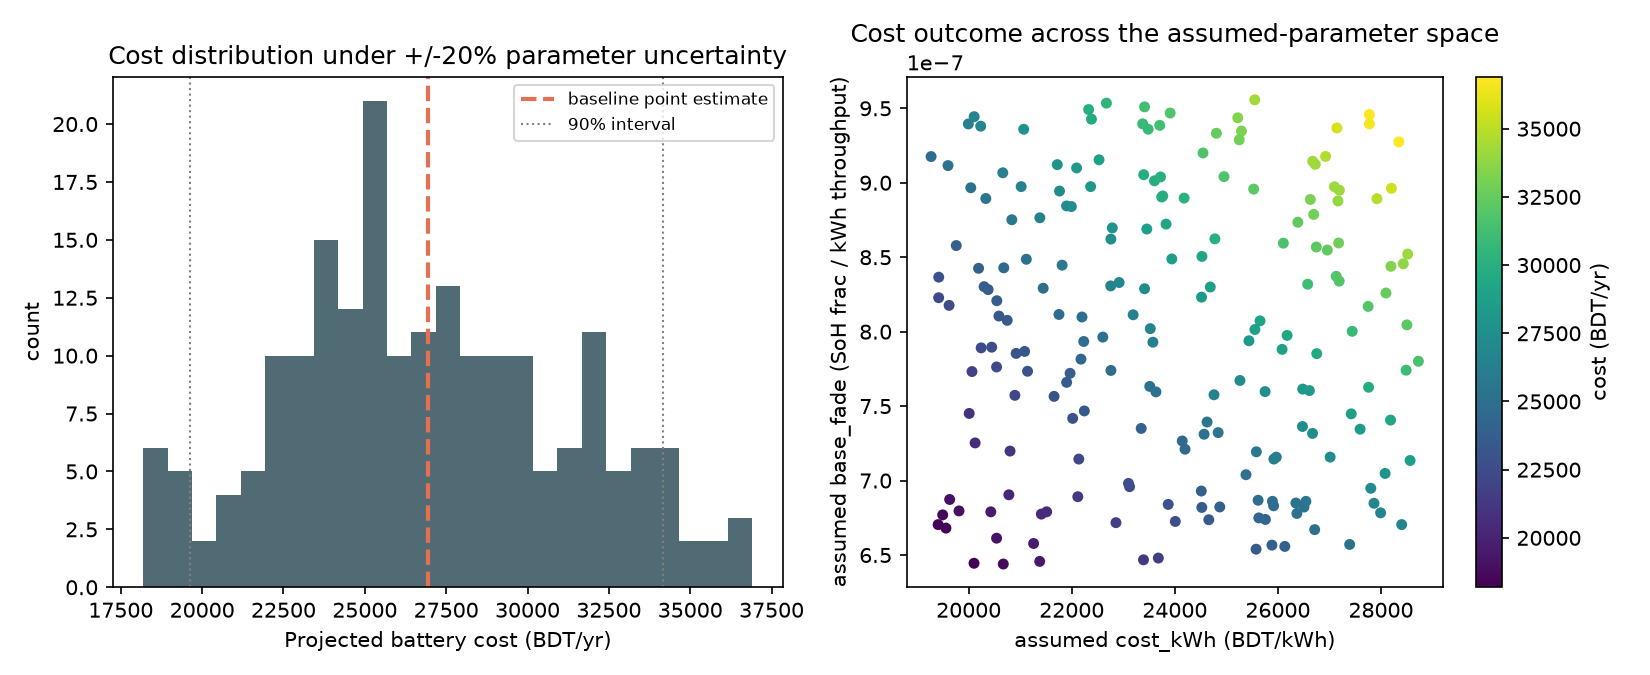
\includegraphics[width=0.85\textwidth]{figs/fig5_cost_sensitivity.png}}
\caption{Battery-cost Monte Carlo under $\pm$20\% assumed-parameter
uncertainty: distribution (left) and outcome across the
assumed-parameter space (right).}
\label{fig:sensitivity}
\end{figure*}

\begin{table}[t]
\centering
\caption{HOMER optimization: three candidate architectures}
\label{tab:homer}
\begin{tabular}{|l|c|c|c|}
\hline
\textbf{Config} & \textbf{Renewable Frac.} & \textbf{COE (\$/kWh)} & \textbf{NPC (\$)} \\
\hline
1 (PV+WT+FC+BESS) & 81.4\% & 0.0278 & 501{,}600 \\
\hline
2 (WT+FC+BESS)     & 53.3\% & 0.0671 & 736{,}617 \\
\hline
3 (FC+BESS only)   & 0.0\%  & 0.1032 & 1{,}120{,}089 \\
\hline
\end{tabular}
\end{table}

\subsection{External Validation}
\label{sec:external-validation}
The twin holds voltage and frequency at an exact constant except
during one scripted sag -- never previously checked against real
telemetry. We compare it to one representative month (April 2023,
259{,}200 valid 10-second samples) of the Mesa Del Sol dataset
\cite{bashir2023mesadelsol}, an unrelated 60~Hz, $\approx$484~V US
microgrid -- only normalized, per-unit behavior is comparable to the
50~Hz, 230~V Jamalpur context. Even with no fault scripted for nearly
the entire month, real frequency shows continuous std
$\approx$0.03\% p.u.\ and real voltage shows continuous std
$\approx$0.5--0.6\% p.u.\ (Fig.~\ref{fig:mesadelsol}) -- concrete
evidence that a constant-V/f-between-events assumption is a real
idealization (Section~\ref{sec:limitations}), not a hand-waved
caveat. This dataset lacks THD/harmonic columns, so it validates V/f
behavior only.

\begin{figure*}[t]
\centerline{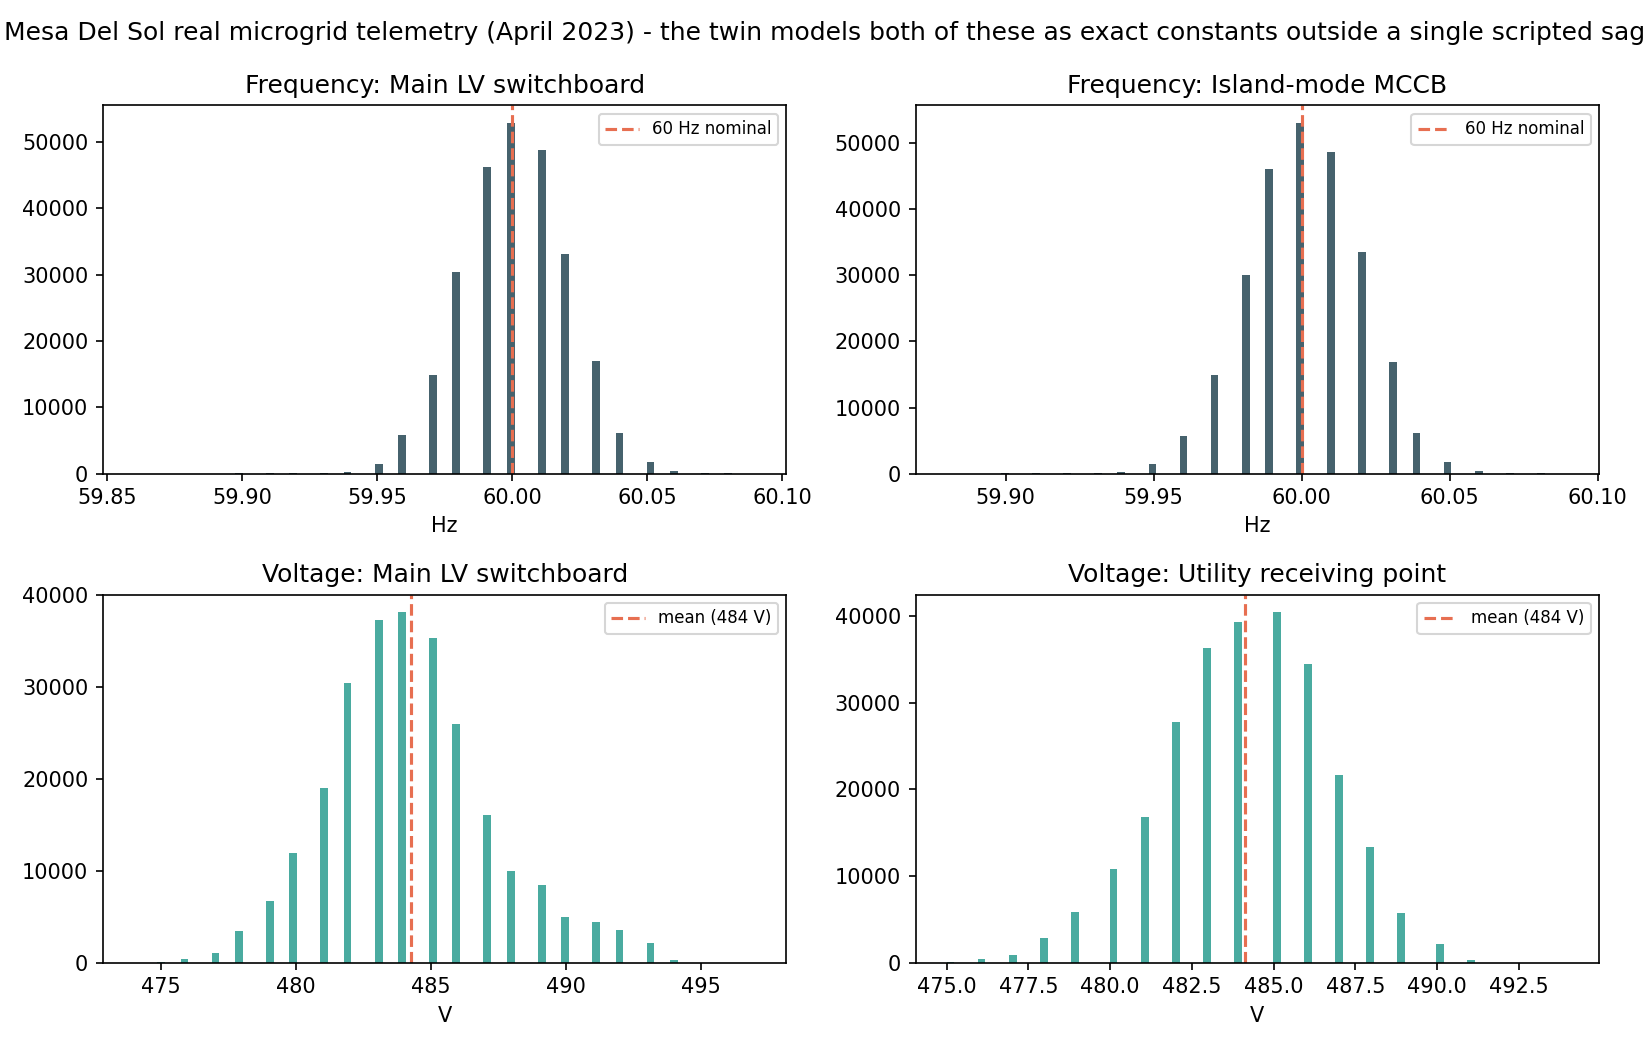
\includegraphics[width=0.85\textwidth]{figs/fig6_mesa_del_sol.png}}
\caption{Independent real-microgrid validation (Mesa Del Sol, April
2023): frequency (top) and voltage (bottom) at two measurement points
each, showing continuous variability absent any scripted event.}
\label{fig:mesadelsol}
\end{figure*}

\section{Results Summary}
Table~\ref{tab:summary} consolidates the headline results; each is
generated by a committed, re-runnable script.

\begin{table}[t]
\centering
\caption{Headline results}
\label{tab:summary}
\begin{tabular}{|p{5.2cm}|c|}
\hline
\textbf{Result} & \textbf{Section} \\
\hline
THD$_i$: 27.13\% $\to$ 2.07\% & \ref{sec:twin} \\
\hline
Disturbance classifier: 99.7\% acc. & III-D \\
\hline
Anomaly detector: ROC-AUC 0.70 vs.\ 0.50 (null control) & III-B \\
\hline
Sim-to-real bridge: 93\% acc. & \ref{sec:bridge} \\
\hline
Cost: 26{,}955 BDT/yr, 90\% CI [19.6k, 34.2k] & \ref{sec:cost} \\
\hline
HOMER: 81.4\% RE $\to$ \$0.0278/kWh & \ref{sec:cost} \\
\hline
External V/f check: real std $\approx$0.03\% (f), $\approx$0.5--0.6\% (V) p.u. & \ref{sec:external-validation} \\
\hline
\end{tabular}
\end{table}

\section{Discussion and Limitations}
\label{sec:limitations}
Several limitations are stated explicitly. The disturbance dataset's
field-measurement provenance rests on an unverified report at the
time of writing; a documentary request is in progress and this
section will be updated once resolved. The near-perfect
disturbance-classification accuracy (99.7\%) is plausible given the
data's low noise and complete sensor coverage, both atypical of field
telemetry, and is reported alongside -- not instead of -- the harder
unsupervised anomaly-detection result (ROC-AUC 0.70) precisely so a
reviewer can weigh both. The 93\% sim-to-real bridge result is, in
this light, meaningful independent evidence: a model cannot be
overfit to idiosyncrasies of a dataset it has never seen, so its
ability to generalize to an unrelated first-principles simulation
signals real learned structure. The twin remains an idealized,
single-branch electrical model (uncited assumed cost parameters,
Simulink cross-validation still pending) that holds V/f at an exact
constant except during one scripted event; Section
\ref{sec:external-validation}'s comparison against an independent
real microgrid confirms this idealization is real, not negligible.

Nothing in this methodology is intrinsically Bangladesh-specific: the
twin's normalized V/f analysis is what let it be validated against an
unrelated US microgrid, and the cost methodology substitutes local
currency/tariff inputs without structural change. This framework is
therefore a candidate response on two fronts: for grids like
Bangladesh's, where 2026 data show the crisis is substantially about
fuel logistics and dispatch reliability rather than installed
capacity \cite{dailystar2026pdbplan,dailystar2026rooppur},
decentralized renewable microgrids reduce dependence on that
constrained centralized supply chain; and for renewable-heavy
developed grids, the same interpretable, cost-aware, cyber-resilient
layer addresses the harmonic and disturbance-management burden that
renewable penetration itself introduces (Section~II). This paper does
not claim to have deployed or field-tested either case -- only that
the methodology does not foreclose either one.

\section{Conclusion}
This paper presented a digital twin framework for renewable-microgrid
power quality management that is cyber-resilient (null-control-
validated anomaly detection), explainable (SHAP attributions matching
power-engineering expectation), and cost-aware (two independent,
uncertainty-quantified cost analyses). Rather than a side-by-side
physics/ML pairing, the two halves were shown to function as one
system: a classifier trained exclusively on real field data correctly
identifies disturbance types in physics-simulated waveforms at 93\%
accuracy, and the twin's own voltage/frequency assumptions were
validated against an independent real microgrid abroad. Future work
includes completing pending Simulink cross-validation, extending the
source-impedance correction into the primary twin rather than the
bridge test alone, and revisiting the dataset-provenance question
once documentary confirmation is available.

\begin{thebibliography}{00}
\bibitem{hernandezmayoral2024pq} E. Hern\'{a}ndez-Mayoral, C. R.
Jim\'{e}nez-Rom\'{a}n, J. A. Enriquez-Santiago, A. L\'{o}pez-L\'{o}pez,
R. A. Gonz\'{a}lez-Dom\'{i}nguez, J. A. Ram\'{i}rez-Torres, J. D.
Rodr\'{i}guez-Romero, and O. A. Jaramillo, ``Power quality analysis of
a microgrid-based on renewable energy sources: A simulation-based
approach,'' \emph{Computation}, vol. 12, no. 11, p. 226, 2024, doi:
\href{https://doi.org/10.3390/computation12110226}{10.3390/computation12110226}.

\bibitem{prakash2025aidcmicrogrid} G. Prakash, R. Dharmaprakash, M. S.
Sujatha, S. Parvez S, and J. K. Reddy, ``Artificial intelligence-based
power management system for a DC micro-grid,'' \emph{Int. J. Electr.
Electron. Eng.}, vol. 12, no. 10, 2025, doi:
\href{https://doi.org/10.14445/23488379/IJEEE-V12I10P109}{10.14445/23488379/IJEEE-V12I10P109}.

\bibitem{jahan2026mlpq} I. Jahan, K. N. D. Dinh, V. Bla\v{z}ek, V.
Snasel, S. Mi\v{s}ak, I. Pergl, F. Mohamed, and A. Mechali, ``Machine
learning-based power quality prediction in a microgrid for community
energy systems,'' \emph{Preprints}, 2026, doi:
\href{https://doi.org/10.20944/preprints202602.1410.v1}{10.20944/preprints202602.1410.v1}.

\bibitem{osifeko2025aiforecasting} M. Osifeko and J. L. Munda,
``AI-based forecasting in renewable-rich microgrids: Challenges and
comparative insights,'' \emph{IEEE Access}, vol. 13, pp. 130446--130474,
2025, doi: \href{https://doi.org/10.1109/ACCESS.2025.3591091}{10.1109/ACCESS.2025.3591091}.

\bibitem{daniel2025dualopt} S. Joshua Daniel, M. Karpagam, A. Flah,
and S. Ben Chaabane, ``Power quality improvement and energy management
in hybrid microgrids using a dual-optimization approach,'' \emph{Sci.
Rep.}, vol. 15, no. 1, p. 36201, 2025, doi:
\href{https://doi.org/10.1038/s41598-025-20001-0}{10.1038/s41598-025-20001-0}.

\bibitem{john2026aipqreview} S. S. John, H. A. Sony, Lavanya V., and
Meera P.S., ``Power quality improvement in microgrids using artificial
intelligence techniques: A review,'' \emph{Sci. Technol. Energy
Transit.}, vol. 81, p. 14, 2026, doi:
\href{https://doi.org/10.2516/stet/2026015}{10.2516/stet/2026015}.

\bibitem{bashir2023mesadelsol} A. Bashir, C. Leap, A. Blumenthal, T.
Estrada, A. Bidram, \emph{et al.}, ``Power, voltage, frequency and
temperature dataset from Mesa Del Sol microgrid,'' \emph{Dryad}, 2023,
doi: \href{https://doi.org/10.5061/dryad.fqz612jzb}{10.5061/dryad.fqz612jzb}.

\bibitem{mbasso2025dtreview} W. F. Mbasso, A. Harrison, I. Dagal, P.
Jangir, M. Khishe, H. Kotb, M. S. Shaikh, A. Smerat, E. Fendzi Donfack,
and R. Kumar, ``Digital twins in renewable energy systems: A
comprehensive review of concepts, applications, and future
directions,'' \emph{Energy Strategy Rev.}, vol. 61, p. 101814, 2025,
doi: \href{https://doi.org/10.1016/j.esr.2025.101814}{10.1016/j.esr.2025.101814}.

\bibitem{barik2025shuntapf} P. K. Barik, G. Shankar, P. K. Sahoo, and
S. Samal, ``Simulation and real-time implementation of a combined
control strategy-based shunt active power filter in microgrid,''
\emph{Sustain. Comput. Inform. Syst.}, vol. 46, p. 101103, 2025, doi:
\href{https://doi.org/10.1016/j.suscom.2025.101103}{10.1016/j.suscom.2025.101103}.

\bibitem{kandula2026xaireview} R. Kandula, J. T. Dandamudi, R. D. A.
Raj, R. M. R. Yanamala, and K. K. Prakasha, ``Explainable AI for smart
grid intelligence: A comprehensive review of techniques, applications
and future directions,'' \emph{Energy AI}, vol. 25, p. 100820, 2026,
doi: \href{https://doi.org/10.1016/j.egyai.2026.100820}{10.1016/j.egyai.2026.100820}.

\bibitem{ahmed2019isolationforest} S. Ahmed, Y. Lee, S.-H. Hyun, and
I. Koo, ``Unsupervised machine learning-based detection of covert data
integrity assault in smart grid networks utilizing isolation forest,''
\emph{IEEE Trans. Inf. Forensics Security}, vol. 14, no. 10, pp.
2765--2777, 2019, doi:
\href{https://doi.org/10.1109/tifs.2019.2902822}{10.1109/tifs.2019.2902822}.

\bibitem{dailystar2026loadshedding} The Daily Star, ``Load shedding
off the charts once again,'' Aug. 2026. [Online]. Available:
\url{https://www.thedailystar.net/news/bangladesh/news/load-shedding-the-charts-once-again-4244141}

\bibitem{dailysun2026rural} Daily Sun, ``2{,}500MW power shortfall
batters rural areas,'' 2026. [Online]. Available:
\url{https://www.daily-sun.com/bangladesh/870461}

\bibitem{dailystar2026pdbplan} The Daily Star, ``PDB's summer power
plan: 60\% capacity of gas plants to stay unutilised,'' Apr. 2026.
[Online]. Available:
\url{https://www.thedailystar.net/news/bangladesh/news/pdbs-summer-power-plan-60-capacity-gas-plants-stay-unutilised-4145386}

\bibitem{dailystar2026rooppur} The Daily Star, ``Bangladesh enters
nuclear energy era,'' May 2026. [Online]. Available:
\url{https://www.thedailystar.net/news/bangladesh/news/bangladesh-enters-nuclear-energy-era-4162461}

\bibitem{tbs2026rooppur} The Business Standard, ``PM may inaugurate
commercial operations of Rooppur nuclear plant in August: Minister
Anam,'' Jun. 2026. [Online]. Available:
\url{https://www.tbsnews.net/bangladesh/energy/pm-may-inaugurate-commercial-operations-rooppur-nuclear-plant-aug-minister-anam}

\end{thebibliography}

\end{document}
